\section{Dados Sensiveis}

\par "Dados como nome, morada e número de contribuinte são mantidos pelo periodo definido por lei após a faturação."\newline

\par "Dados pessoais necessários para realizar candidaturas ou donativos são também guardados até ao final do processo para os quais foram dados. Após isso são eliminados."\newline

\par Por estas citações podemos concluir que caso ganhemos aceso ao sistema, conseguiremos obter nomes, moradas, números de contribuintes e outros dados sensiveis.



\subsection{Fragilidades na Comunicação de Dados Pessoais e Segurança}


\par "A Companhia recorre a parceiros externos nomeadamente para desenvolvimento, manutenção e alojamento de sistemas informáticos, agências de marketing e comunicação, estudos de mercado, apoio ao cliente, a triagem, avaliação e selecção de candidatos. Nestes casos, a Companhia assegura que os seus parceiros cumprem com as medidas técnicas e organizacionais adequadas à actividade de processamento. Neste âmbito, os dados recolhidos poderão ser transferidos para entidades que se localizam em países terceiros (fora da União Europeia), sendo assegurado que são tomadas as medidas de segurança apropriadas de acordo com a legislação em vigor."\newline


\par Segundo esta citação os dados pessoais dos utilizadores podem ser enviados a terceiros aumentando as chances de um atacante poder obter esses dados durante a transferência dos mesmo. Para além disso as politicas de segurança de uma empresa "parceira" do pingo doce ainda que submetida á legislação em vigor, pode ter critérios de segurança pouco firmes por exemplo no requisito de impedir ataques por engenharia social.\newline
\par Note-se que uma das melhores formas de obter dados sensiveis de uma empresa de grande dimensão é muitas vezes fazendo uso de parceiros de menor dimensão com critérios de segurança mais lassos.


\section{Autenticação - Facebook ou Google}

\par O utilizador da plataforma pode usar uma conta Google ou de Facebook para se autenticar na plataforma, isto acrecenta vulnerabilidades no acesso aos dados do utilizador visto que podemos atacar outros sistemas para além deste, que podem ter outras vulnerabilidades.
\par Por exemplo, o facebook, caso um utilizador se engane a escrever a password e apenas altere uma letra muitas vezes assume que se trata da pessoa certa e permite o acesso á conta.



\section{Contactos Importantes}
\begin{itemize}
\item Correio electrónico para clientes: cliente@pingodoce.pt\newline


\item Telemóvel: 808 204 545 \newline


\item Telefone:  210 114 411\newline


\item Linha de registo cartão poupa mais: 707 50 20 69\newline

\item Localização sede:\newline


\par Av. Santo Condestável – Via Central Chelas 1900-806 Lisboa\newline


\item Localização do departamento de recursos humanos: \newline


\par Pingo Doce Distribuição Alimentar SA., Rua Actor António Silva, 7 – 6º 1649-033 Lisboa \newline

\item CEO pingo doce: Isabel Ferreira Pinto\newline

\par Perfil Linkdin: https://www.linkedin.com/in/isabel-ferreira-pinto-73b88046/\newline

\item Perfis de funcionários úteis para "social engeniering":\newline

\par https://www.linkedin.com/company/pingo-doce/people/\newline

\item Email do encarregado de Protecção de Dados:  dpo.portugal@jeronimo-martins.com \newline
\end{itemize}


\section{Querys para obter informações sobre servidores e serviços}

\subsection{dig -4 www.pingodoce.pt}

\flushleft{
;; OPT PSEUDOSECTION: \newline
; EDNS: version: 0, flags:; udp: 4096 \newline
;; QUESTION SECTION: \newline
;www.pingodoce.pt.		IN	A \newline


;; ANSWER SECTION: \newline
www.pingodoce.pt.	44	IN	A	194.65.31.215 \newline


;; AUTHORITY SECTION: \newline
pingodoce.pt.		44	IN	NS	dns3.pingodoce.pt. \newline
pingodoce.pt.		44	IN	NS	dns2.pingodoce.pt. \newline
pingodoce.pt.		44	IN	NS	dns.pingodoce.pt. \newline


;; ADDITIONAL SECTION: \newline
dns3.pingodoce.pt.	44	IN	A	213.13.169.10 \newline
dns.pingodoce.pt.	44	IN	A	194.65.31.202 \newline
dns2.pingodoce.pt.	44	IN	A	194.65.31.203 \newline


;; Query time: 52 msec \newline
;; SERVER: 193.137.16.65\#53(193.137.16.65) \newline
;; WHEN: Mon Oct 28 10:05:15 WET 2019 \newline
;; MSG SIZE  rcvd: 165 \newline
}
\indent\rule{8cm}{0.4pt}

\par Note-se que só é apresentado o dig -4 e não o dig -6 pois não há resposta de nenhum servidor quando inquirimos www.pingodoce.pt com IPv6.\newline
\par Como podemos ver pela resposta obtida pelo dig temos 3 NameServers autoritários para \textit{www.pingodoce.pt}:
\begin{itemize}
\item dns3.pingodoce.pt
\item dns2.pingodoce.pt 
\item dns.pingodoce.pt
\end{itemize}


\par Estes têm respetivamente os seguintes endereços IPv4:
\begin{itemize}
\item 213.13.169.10
\item 194.65.31.203
\item 194.65.31.202
\end{itemize}


\par O endereço destino \textit{www.pingodoce.pt} tem IPv4 194.65.31.215.\newline


\par Podemos concluir sobre os IPs que dois dos nomes autoritários partilham a mesma rede do endereço alvo (194.65.31.X/24) e um terceiro servidor, dns3.pingodoce.pt, encontra-se numa rede separada (213.13.169.X/24).

\subsection{Whois pingodoce.pt}

\flushleft{
Domain: pingodoce.pt\newline
Domain Status: Registered\newline


Creation Date: 04/06/1998 00:00:00\newline
Expiration Date: 04/07/2022 23:59:40\newline


Owner Name: Pingo Doce - Distribuicao Alimentar S.A.\newline
Owner Address: Rua Actor Antonio Silva, 7\newline
Owner Locality: LISBOA\newline
Owner ZipCode: 1649-033\newline
Owner Locality ZipCode: LISBOA\newline
Owner Country Code: PT\newline
Owner Email: dsiaccounts@jeronimo-martins.pt,dsiaccounts@jeronimo-martins.com\newline


Admin Name: Pingo Doce - Distribuicao Alimentar S.A.\newline
Admin Address: Rua Actor Antonio Silva, 7\newline
Admin Locality: LISBOA\newline
Admin ZipCode: 1649-033\newline
Admin Locality ZipCode: LISBOA\newline
Admin Country Code: PT\newline
Admin Email: dsiaccounts@jeronimo-martins.pt,dsiaccounts@jeronimo-martins.com\newline


Name Server: dns2.pingodoce.pt | IPv4: 194.65.31.203 and IPv6: \newline
Name Server: dns3.pingodoce.pt | IPv4: 213.13.169.10 and IPv6: \newline
Name Server: dns.pingodoce.pt | IPv4: 194.65.31.202 and IPv6: \newline
}

\noindent\rule{8cm}{0.4pt}

\par Com o comando \textit{whois pingodoce.pt} obtemos mais algumas informações sobre quem estamos a investigar.\newline
Estas informações são sobre as datas de criação e em que expira o dominio, sobre o dono sabemos o nome, a localização da sua sede, o código postal, o pais e o email do mesmo. Para além disso temos análogas sobre o administrador do sistema.\newline
Apesar de usar o whois nos fornecer estes dados extra de formos a \url{https://www.iana.org/whois} e pesquisarmos por \textit{www.pingodoce.pt} podemos obter informação sobre quem registou este site, neste caso os responsáveis pelo dominio \textit{.pt}. O resultado segue em baixo.

\begin{figure}[H]

	\centering

 	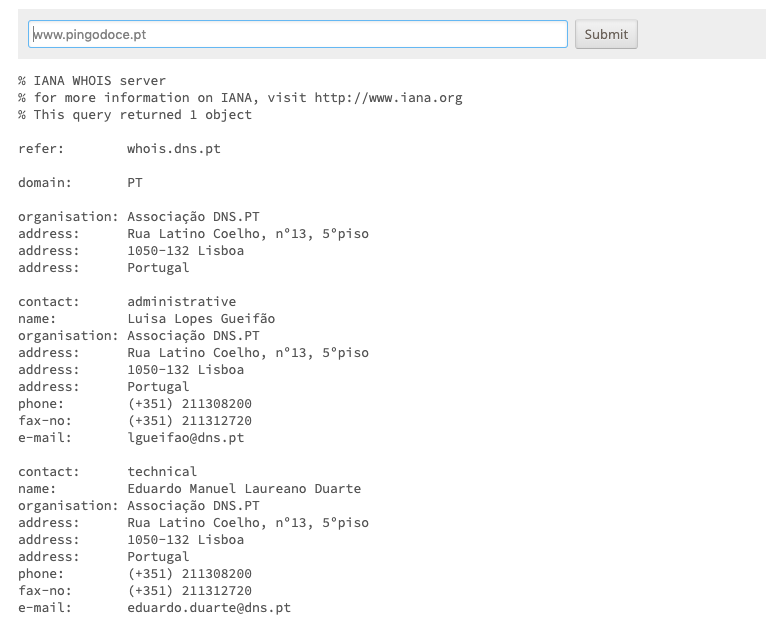
\includegraphics[scale = 0.5]{registadorPingoDoce1.png}
 	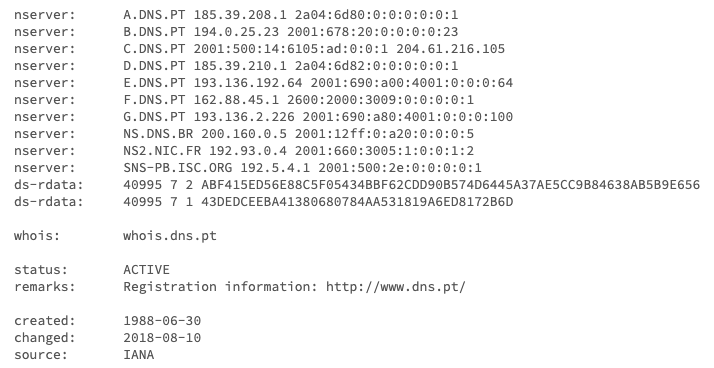
\includegraphics[scale = 0.5]{registadorPingoDoce2.png}
 	\caption {Dados do registador do site www.pingodoce.pt}

  	\label{fig01}
\end{figure}


Este resultado é útil na medida em que revela nomes, emails, números de telefone etc.

Posteriormente foram testadas algumas portas para o IP 194.65.31.215 referente a www.pingodoce.pt. A seguinte imagem representa a busca feita a várias portas conhecidas que se enumeram de seguida bem como os respetivos resultados.

\begin{figure}[H]

	\centering

 	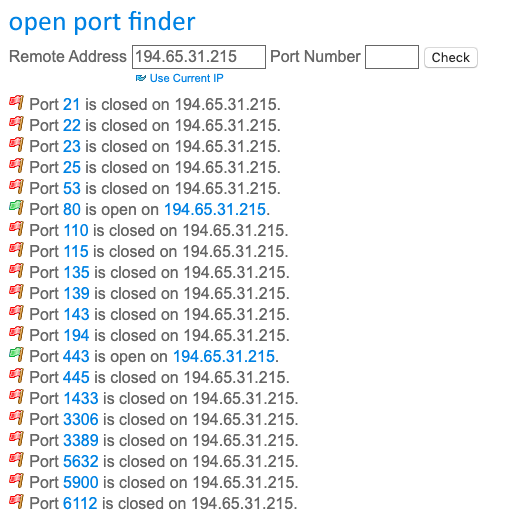
\includegraphics[scale = 0.6]{portsCheck.png}
 	\caption {Exemplo de teste feito a portas do IPv4 correspondente a www.pingodoce.pt}

  	\label{fig:02}
\end{figure}

\par \textbf{Portas testadas:} 
\begin{itemize}
\item FTP
\item SSH
\item TELNET
\item SMTP
\item DNS
\item HTTP
\item POP3
\item SFTP
\item RPC
\item netBIOS
\item IMAP
\item IRC
\item SSL
\item SMB
\item MSSQL
\item MySQL
\item RemoteDesktop
\item PCAnywhere
\item VNC
\item Warcraft III
\end{itemize}

\par Com esta análize podemos concluir que tanto o HTTP como o SSL têm as respetivas portas abertas.\newline


\par Determinar o endereço de email é uma forma de localizar a firewall da organização, para isso basta usar -textit{host pingodoce.pt}. O resultado pode ser visto na figura abaixo.

\begin{figure}[H]

	\centering

 	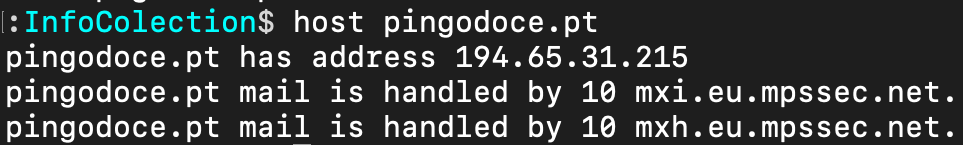
\includegraphics[scale = 0.4]{hostMailHandler.png}
 	\caption {Emails referentes a pingodoce.pt}

  	\label{fig:03}
\end{figure}

\par Por fim, fazendo uso do nmap sobre o ip referente a pingodoce.pt obtemos as seguintes imagens.
 \begin{figure}[H]

	\centering

 	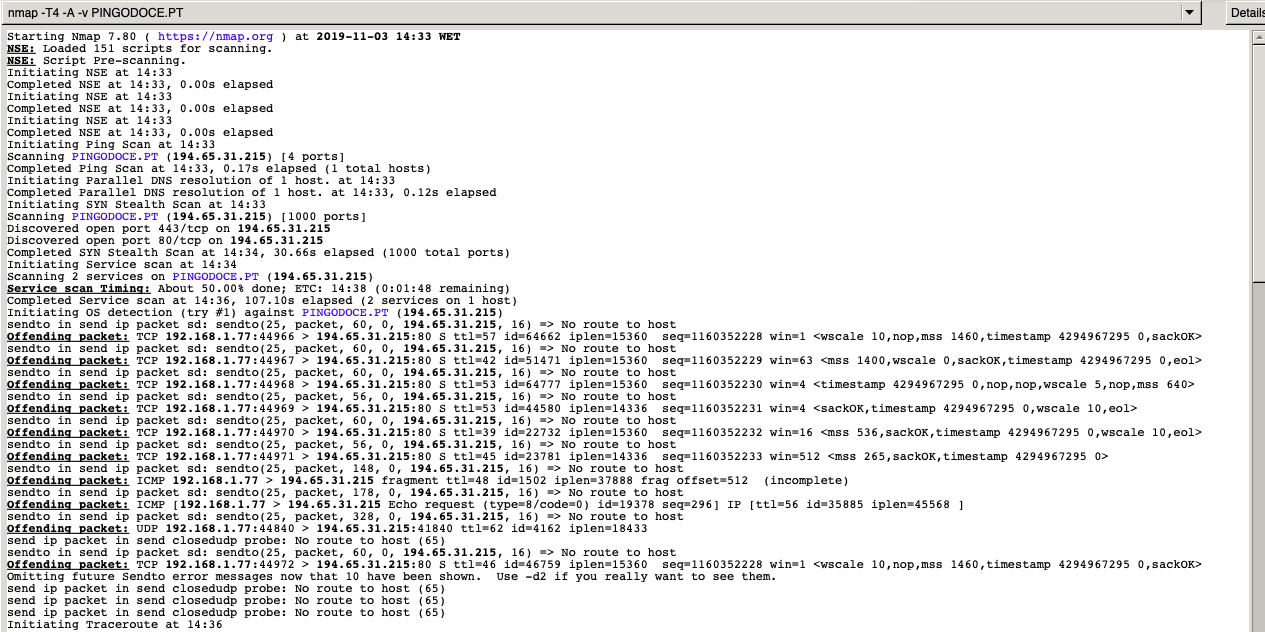
\includegraphics[scale = 0.4]{NMAPscan1.png}
 	\caption {NMAP output 1}

  	\label{fig:04}
\end{figure}
\begin{figure}[H]

	\centering

 	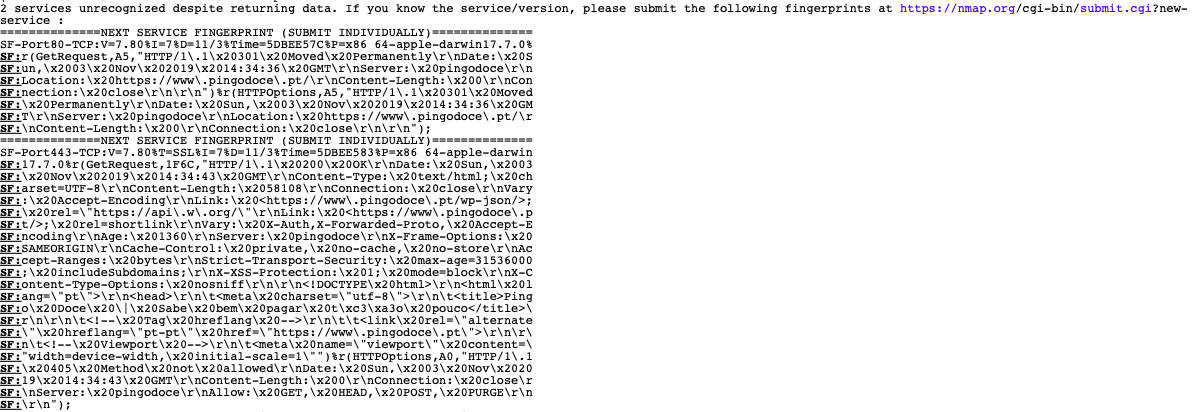
\includegraphics[scale = 0.4]{NMAPscan2.png}
 	\caption {NMAP output 2}

  	\label{fig:05}
\end{figure}

\par Na primeira podemos inferir que deve haver uma firewall ou um mecanismo de segurança a bloquear os acessos ao servidor, isto porque para cada pacote enviado é retornado o resultado \textit{No route to host}.\newline
\par Na segunda imagem temos a resposta de dois serviços não identificados, este podem possívelmente ser explorados caso descubramos a sua identidade.\newline
\par Resumindo toda a informação obtida sobre o Pingo Doce ao longo deste trabalho, a empresa tem uma postura de segurança boa em relação á manutenção de servidores, precavem-se contra possíveis ataques de DoS e em termos de acesso a informação sensivel sobre a rede interna da empresa. No entanto peca na vertente da engenharia social, a informação de quem são os empregados é pública e estes não uma fonte de preocupação em termos de segurança visto que na maior parte das vezes estes são a porta de entrada para um sistema. 

